
\chapter{Data-to-Text Generation with Custom Datasets}
\label{chap:investigating}

In this chapter, we observe and quantify behaviors of neural \acp{lm} in specific \ac{d2t} generation scenarios. To support our investigations, we venture beyond existing \ac{d2t} generation datasets.
% There are several reasons why existing datasets may not be adequate: low variability of data labels, inadequate formats, or the issues with data contamination. 
Building custom datasets helps us to overcome limitations of existing datasets and provide a more detailed picture for the task we set out to study.

In \autoref{sec:rel2text}, we examine the capabilities of \acp{plm} to describe relations between entities in knowledge graphs. As we note, existing datasets were not able to discern memorization from generalization. We thus collect a custom dataset with a large variety of relation labels, including unseen labels in the test set. Using our dataset, we investigate whether the models can correctly describe the relations they have not seen in the training data. We find out that the models can generalize unseen labels as long as the labels are human-readable and unambiguous, which is often (but not always) fulfilled in real-world data.

In \autoref{sec:quintd}, we investigate abilities of open \acp{llm} for \ac{d2t} generation. To prevent data contamination, we scrape unlabeled data from public sources across five domains. As the data is in common formats that the models have seen during pretraining, we can evaluate the ability of the models to describe the data in zero-shot settings. Using \ac{llm}-based referenceless metric and human annotators, we quantify the semantic accuracy of the generated texts with respect to the input data. We find out that although the descriptions are fluent, large majority of them contains semantic errors. We also provide practical recommendations for \ac{d2t} generation in similar scenarios.

\section{Describing Relations in Knowledge Graphs}
\label{sec:rel2text}
\begin{refbox}
    This section is based on the paper \emph{Mind the Labels: Describing Relations in Knowledge Graphs With Pretrained Models} \cite{kasnerMindLabelsDescribing2022}, joint work with Ioannis Konstas and Ondřej Dušek. The work was published in the Proceedings of the 17th Conference of the European Chapter of the Association for Computational Linguistics (EACL 2023). The project was led by the author of the thesis; Ioannis Konstas and Ondřej Dušek mentored the project.
\end{refbox}
In this section, we investigate to which extent do human-readable data labels help \acp{plm} with \ac{d2t} generation. We start by noticing that \acp{plm} can use labels such as column headings, keys, or relation names to generalize to out-of-domain examples. However, is this ability robust enough, and do we also expect the models to produce accurate outputs if these labels are ambiguous or incomplete?

Specifically, we focus here on the task of descibing a relation between two entities. For our experiments, we collect \textsc{Rel2Text}: a novel dataset for verbalizing a diverse set of 1,522 unique relations from three large-scale knowledge graphs (Wikidata, DBPedia, YAGO). We evaluate model outputs on unseen relations using a combination of automatic metrics and manual analysis. We find that although PLMs for D2T generation expectedly fail on unclear cases, models trained with a large variety of relation labels are surprisingly robust in verbalizing novel, unseen relations. We argue that using data with a diverse set of clear and meaningful labels is key to training D2T generation systems capable of generalizing to novel domains. We release the code and data for our experiments on Github.\footnote{\url{https://github.com/kasnerz/rel2text}}


% 
% In this paper, 

\subsection{Motivation}
D2T generation systems need to accurately capture the semantics of relations between values in the data. However, the data labels such as relation names \cite{farber2018linked,haller2022analysis}, table headings \cite{parikhToTToControlledTableToText2020}, or meaning representation keys \cite{dusekEvaluatingStateoftheartEndtoEnd2020} may provide only superficial or---if the labels are abbreviations, such as in the Rotowire dataset \cite{wiseman2017challenges}---no usable hints about the data semantics. Learning how to properly describe the data is thus a challenge for \ac{d2t} generation systems, typically requiring in-domain training data of sufficient quality and quantity \cite{dusekSemanticNoiseMatters2019}.

PLMs such as BART \cite{lewisBARTDenoisingSequencetoSequence2019} or T5 \cite{raffelExploringLimitsTransfer2019} can quickly adapt to new domains and exhibit robustness to out-of-domain inputs. However, the PLMs for D2T generation are still limited by the expressivity of the data labels. Consider \autoref{fig:rel2text:teaser} (a): the model can use its representation of \textit{``godparent''} to understand there is a \textit{``is-a-godparent-of''} relation between the entities, but it has to infer (or guess) who is the godparent of whom. Even in the less ambiguous cases (b) and (c), the model still has to correctly capture the intended semantics of the relation (e.g. \textit{``occupant''} meaning \textit{``home team''}).


\begin{figure}[t]

    \begin{minipage}{0.55\textwidth}
        \centering
        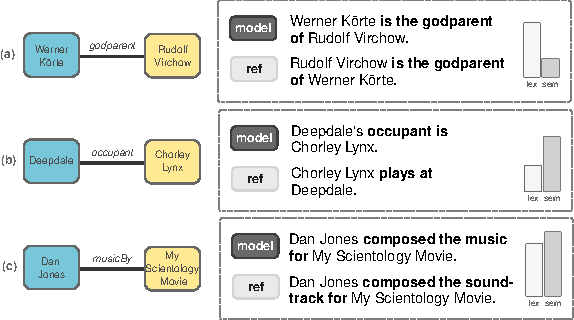
\includegraphics[width=\textwidth]{img/mind_the_labels.pdf}
        \caption{Data-to-text generation models use relation labels (such as  \mbox{\textit{godparent}}, \mbox{\textit{occupant}}, and \mbox{\textit{musicBy}}) to describe relations between entities. However, unclear labels can lead to various lexical or semantic incoherencies in the output descriptions, such as swapping the relation direction (a), using too literal expressions (b), or expressions with low specificity.}
        \label{fig:rel2text:teaser}
    \end{minipage}
    \hfill
    \begin{minipage}{0.4\textwidth}
        % \begin{table}[t!] \footnotesize
        % \def\arraystretch{1.2}
        \centering
        \footnotesize
        \begin{tabular}{lp{3.3cm}} \toprule
            \textbf{relation}   & \textbf{verbalization}                                               \\ \midrule
            \textit{is part of} & \eh{} is part of \et{}.                                              \\\hdashline[0.5pt/2pt]
            \textit{duration}   & \eh{} lasted for \et{}.                                              \\\hdashline[0.5pt/2pt]
            \textit{platform}   & \eh{} is available on \et{}.\newline\eh{} runs on \et{}.             \\\hdashline[0.5pt/2pt]
            \textit{country}    & \eh{} was born in \et{}. \newline \eh{} is located in \et{}.         \\\hdashline[0.5pt/2pt]
            \textit{parent}     & \eh{} is the parent of \et{}. \newline \et{} is the parent of \eh{}. \\\bottomrule
        \end{tabular}
        \captionof{table}{Example verbalizations of relation labels with head and tail entities (\eh, \et). Relations can be copied verbatim (\textit{is part of}), have a unique verbalization (\textit{duration}), or multiple equivalent lexical choices (\textit{platform}). There %may also be 
            is also ambiguity stemming from the semantics of the entities (\textit{country}) or the relation itself (\textit{parent}).}
        \label{tab:example}
        % \end{table}
    \end{minipage}
\end{figure}

We investigate to what extent can PLMs use arbitrary labels describing relations between entities. A suitable testing ground is the task of describing (i.e., \textit{verbalizing}) individual triples in a \ac{kg}, which can be considered a trivial case of graph-to-text generation \cite{ribeiroInvestigatingPretrainedLanguage2020,koncel-kedziorskiTextGenerationKnowledge2019}. In this task, there is a wide range of lexical choices for the \textit{relation label} (see Table \ref{tab:example}), while the \textit{entities} can be copied verbatim or with only minor morphological changes.

Current human-annotated datasets for D2T generation contain only a small number of relations
%(ranging from a handful to lower hundreds) 
and rarely contain any unseen relations in the test set \cite{mille2021automatic}.
We collect a novel dataset \textsc{Rel2Text} (\underline{R}e-writing \underline{e}dge \underline{l}abels to Text),\footnote{Or simply ``Relations-to-Text''.} acting as a test bench for our experiments. It contains 4,097 single triples from three large-scale KGs (Wikidata, \mbox{DBPedia}, and YAGO) and their crowdsourced verbalizations, covering 1,522 unique relations (§\ref{sec:data}). Each relation is equipped with a label, a textual description, and up to five triples in which the relation occurs in the KG.

Using the \textsc{Rel2Text} dataset, we evalute the ability of PLMs to verbalize relations which were not present in the training set. We consider both models finetuned on other relations in our dataset and models finetuned on datasets from a related domain. We also experiment with scenarios involving few-shot finetuning, training on masked labels, and extending the labels with descriptions (§\ref{sec:analysis},~\ref{sec:results}).

We find that the PLMs are quite robust in verbalizing a diverse set of relations based on their label (achieving \textasciitilde 90\% of overall entailment probability). We show that semantically unfaithful model outputs are often caused by incomplete, ambiguous, or noisy input data. Somewhat suprisingly, we also show that longer relation descriptions do not provide substantial improvements over using short labels. However, even for data using short relation labels, the model trained on verbalizing relations can achieve results comparable to verbalizing relations using manual templates in two downstream tasks (§\ref{sec:downstream}).





The contributions of our work are as follows:
\begin{itemize}
    \item We examine the ability of PLMs to describe graph relations, showing that \textit{clear and meaningful labels} are the basis for successful generalization to unseen relations.
    \item We present \textsc{Rel2Text}---a human-annotated dataset with 4,097 examples verbalizing 1,522 relations from three large-scale open KGs.
    \item We show that a model trained on \textsc{Rel2Text} can serve as a drop-in replacement for manual templates, preserving or improving performance on downstream tasks.
\end{itemize}




\section{Describing Data in Common Formats}
\label{sec:quintd}